\chapter{WagonSim}
\label{ch:wagonSim}
% ##################################################################################################################

\hfill \textbf{Author:} ... Balmi fragen

\begin{center} 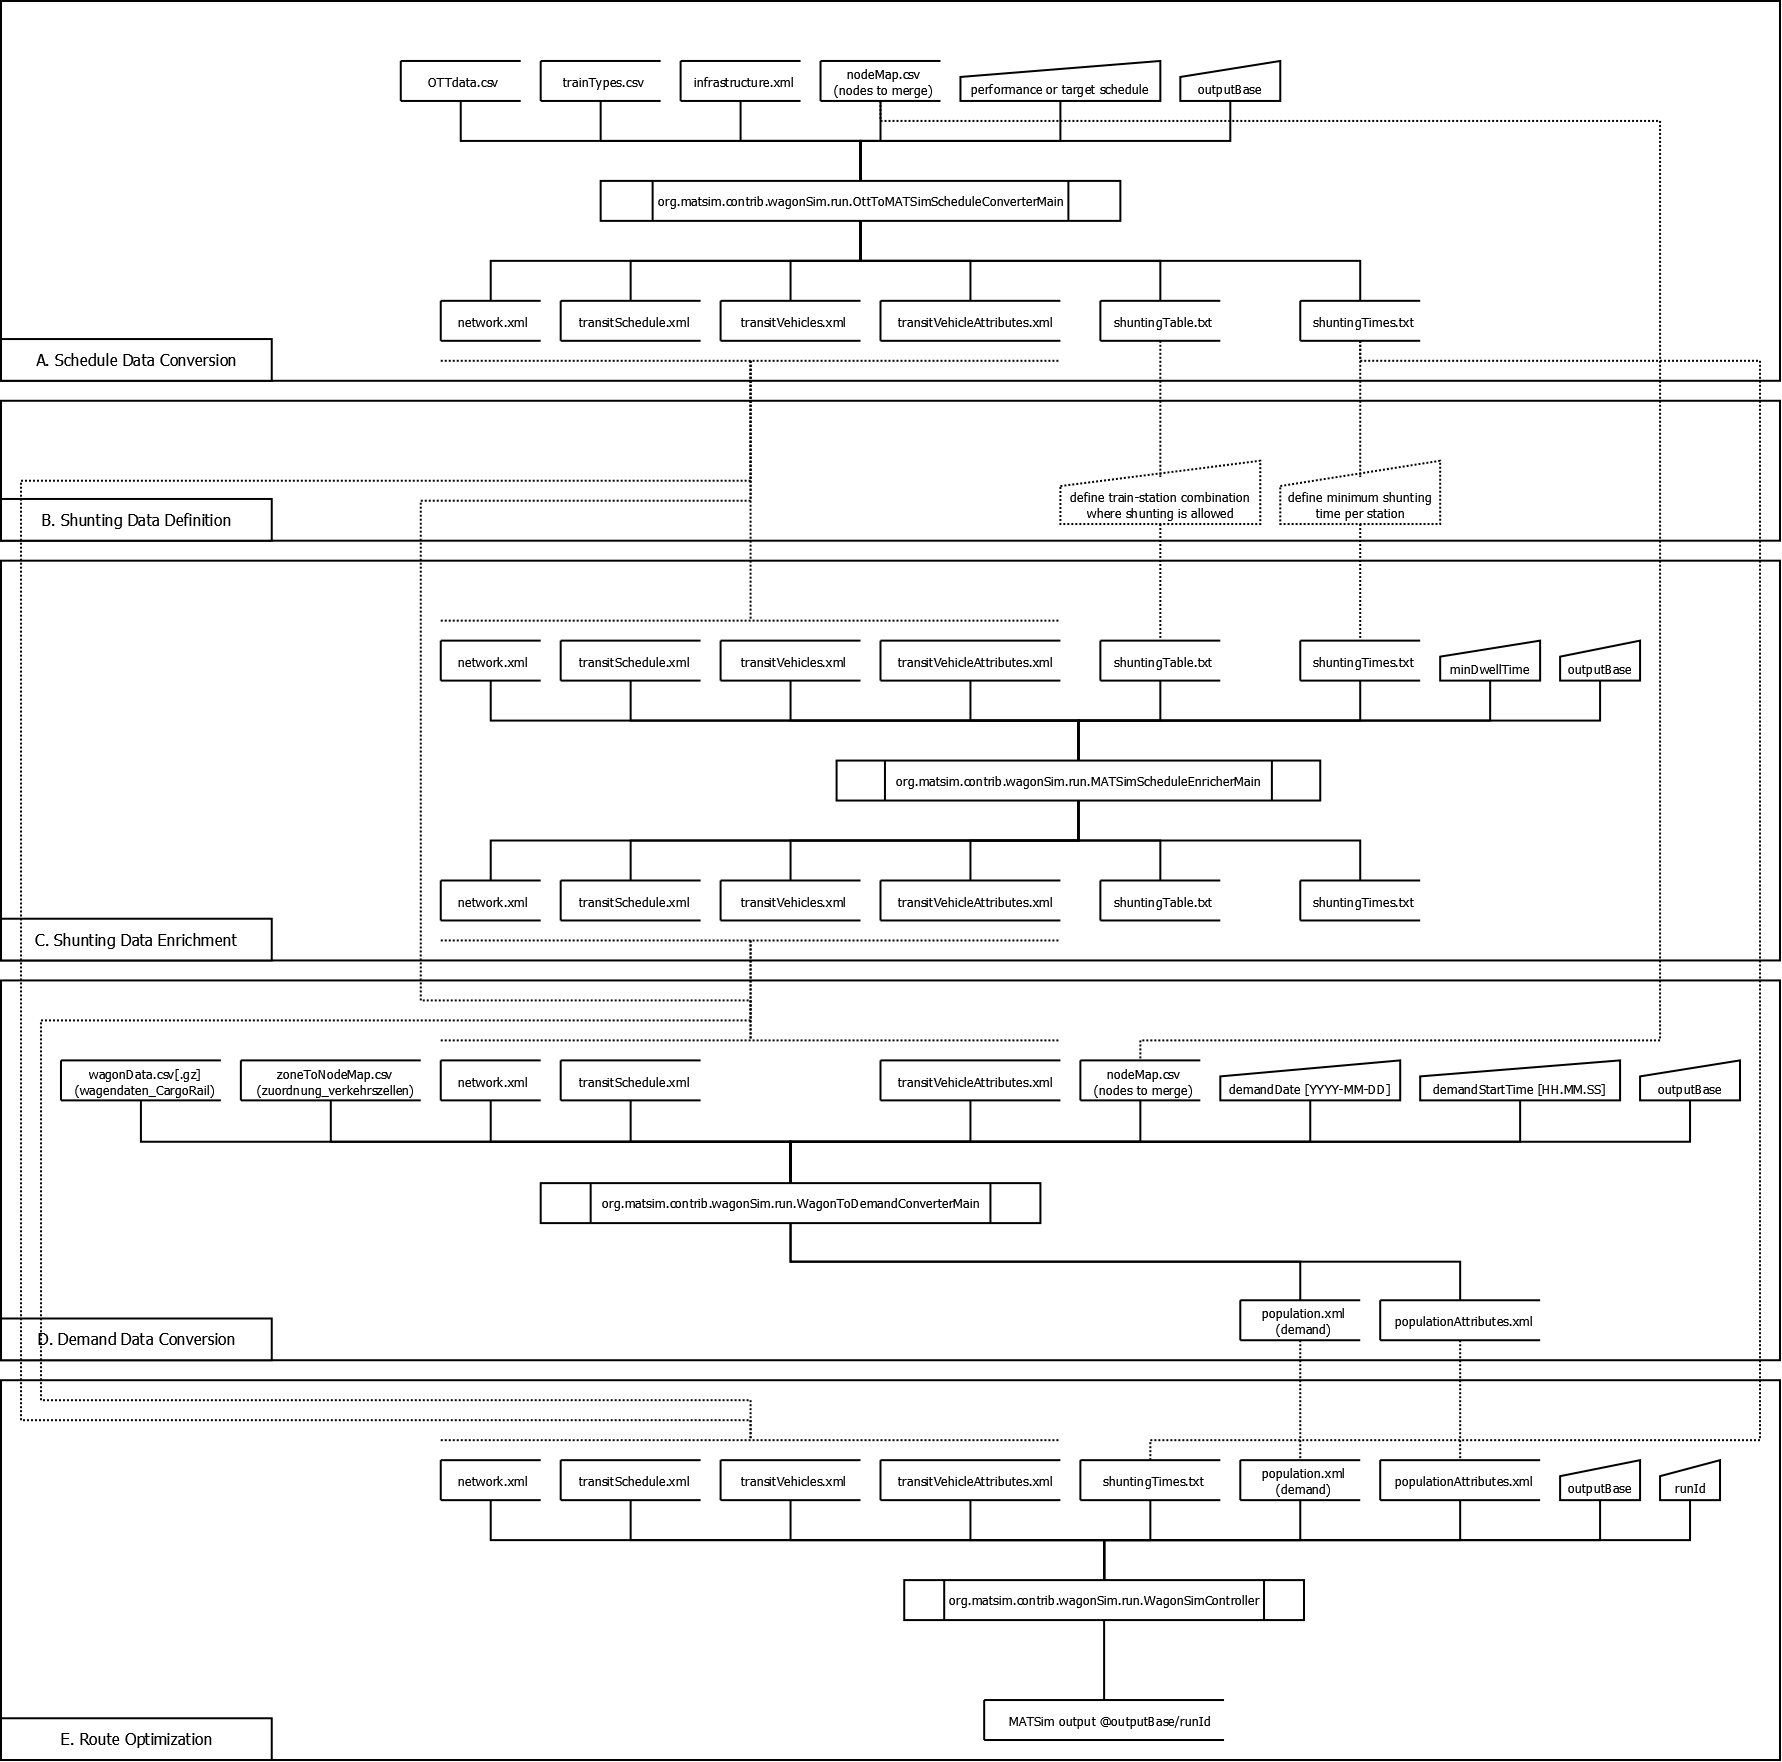
\includegraphics[width=0.25\textwidth, angle=0]{extending/figures/wagonsim/wagonSimProcessChain.png} \end{center}

\createStandardInformation{wagonSim}{\lstinline|WagonSimController| class}{todo}{-}

% ##################################################################################################################
\ah{taken from \url{http://www.matsim.org/extensions/wagonSim} and slightly adapted}
The wagonSim \gls{contribution} allows one to use \gls{matsim}'s route-optimization process to find the optimal paths for rail-based freight wagons on a given rail-based freight infrastructure.

The network links here define the rails, the nodes define the train stations and the schedule transit stops defines the train station stopping points. Freight locomotives are driven by on a strictly fixed schedule where each locomotive is given as a single transit line with a single transit route and a single departure. The freight wagons correspond to agents with a given origin and destination (single trip agents). Routing takes various constraints into account, \ie a minimum shunting time while switching locomotives, maximum weight and length of a freight train and it differentiates between locomotive stops for shunting and stops for just waiting (without the possibility for shunting).

wagonSim \gls{contribution} is based on specialized input data. First step is input data conversion into \gls{matsim} formats (scenario data). Second it allows one to manually adapt the scenario for different parametrization of train stops, shunting stations, minimum shunting times and dwell times of trains at stops. And third it sets up the configuration of the route optimization and runs the \gls{matsim} optimization cycle.

As shown at shown at \url{http://www.matsim.org/docs/extensions/wagonSim} and in Figure~\ref{fig:wagonSimProcessChain} data conversion and wagonSim execution is composed of five stages, described in more detail at above referenced url.
%
\begin{enumerate}[(A)]
\item Schedule data conversion
\item Shunting data definition
\item Shunting data enrichment
\item Demand data conversion
\item Route optimization
\end{enumerate}
%
The wagonSim \gls{contribution} has been applied for projects of the \gls{eth}, \gls{ivt} Transport Systems group.

\createfigure%
{WagonSim process chain}%
{WagonSim process chain}%
{\label{fig:wagonSimProcessChain}}%
{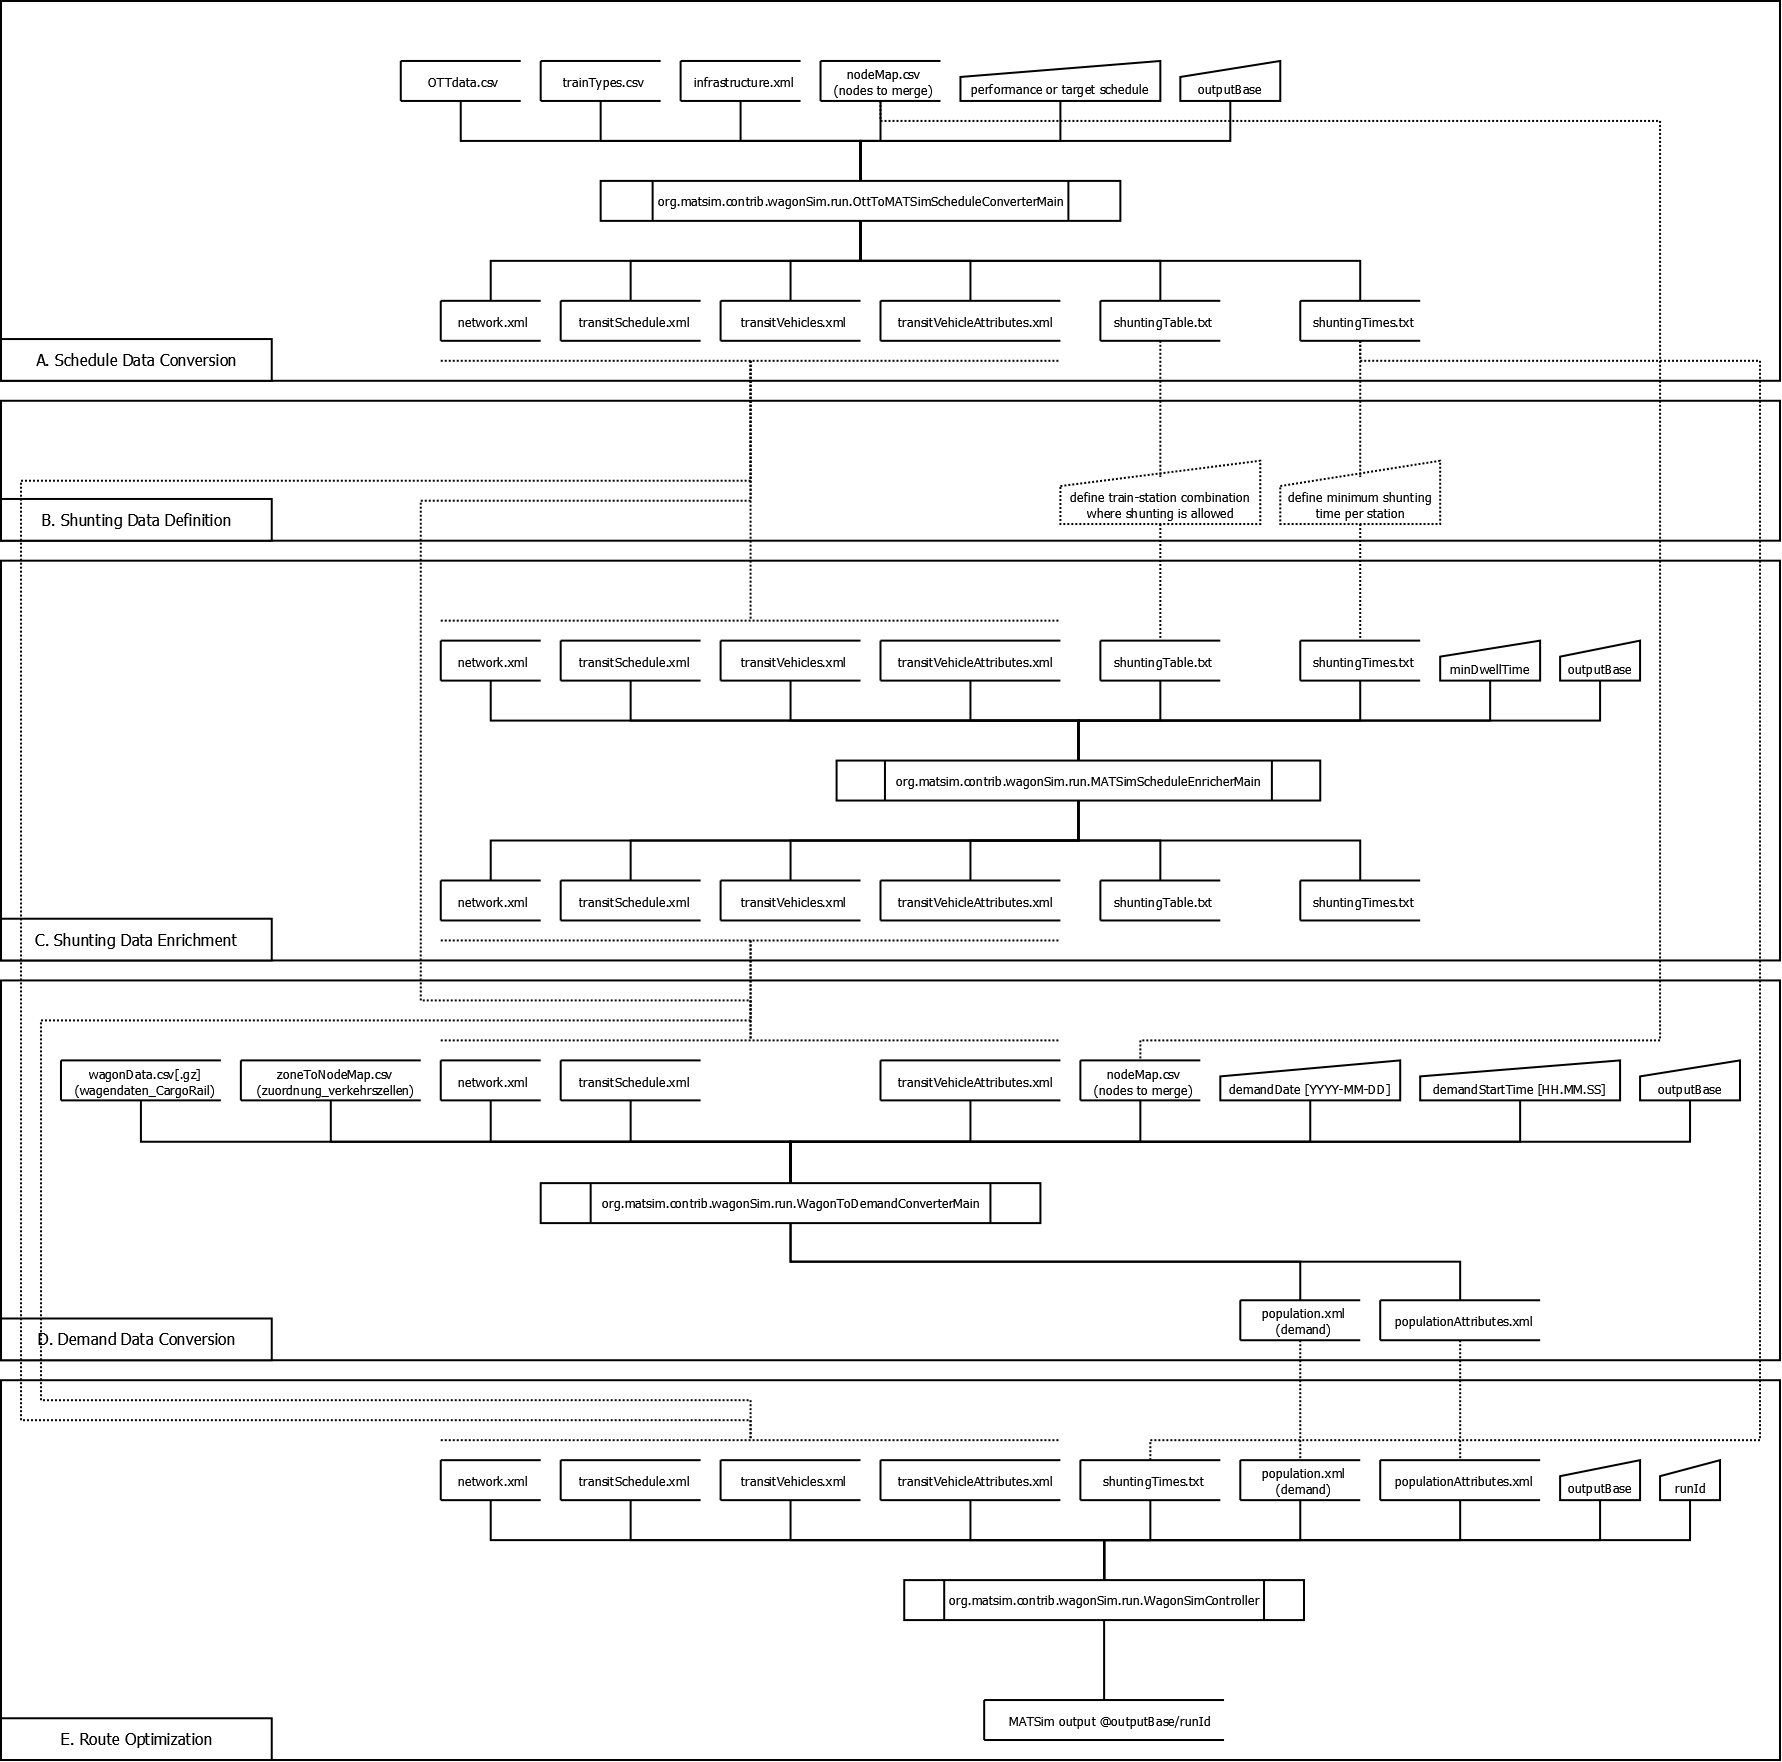
\includegraphics[width=1.\textwidth,angle=90]{extending/figures/wagonsim/wagonSimProcessChain.png}}%
{}

% ##################################################################################################################